% CREATED BY DAVID FRISK, 2016
\chapter{Model}
The simulation is at the essence a particle-based model, where spherical particles are used to represent entities analogous to biological cells, both dead and living, as well as energy particles. This chapter will describe the model; including the physics implemented to handle the particle interactions as well as the evolutionary and organism-related structures created around them.
\section{Particle-based physics}
Each particle has properties such as position, velocity, force, radius, density and energy level, which are accessible and modifiable in the interaction functions.

\subsection{Particle types} \label{subsec:particleTypes}
There are four particle types implemented in the model: \emph{Cells}, \emph{Detritus}, \emph{Buffer} and \emph{Energy particles}.
\begin{description}
    \item [Cell] The cell particle is analogous to the biological cell, although a significant simplification. Apart from the ordinary particle properties, a cell also has knowledge of which organism it belongs to (by an organism ID), which cells are its neighbours, and what type of cell it is. Neighbouring cells will, while in contact, exchange energy with each other, where the amount being exchanged depends on the cell types.
    \item [Detritus] When a cell less energy than the predefined amount \emph{minCellEnergy}, the cell dies and turns into a detritus particle. All detritus are dead cells and might have an energy amount larger than \emph{minCellEnergy} if it died of other causes than energy deprivation. Over time, the detritus decays, losing energy, until none is left and the particle disappears (turns into a buffer particle).
    \item [Buffer particle] A limitation with the Fluidix library is that increasing the number of particles is a costly operations. Because of this, the model keeps a constant number of particles at all times. The ones not currently in use are set as buffer particles and positioned outside the simulation boundaries. 
    \item [Energy particle] In order to provide energy to the system, the model includes energy particles constantly falling down from the sky. Each particle contains a predefined amount of energy, which upon contact with a photosynthetic cell gets transferred to the cell while the energy particle turns into a buffer particle.
\end{description}
\begin{figure}
  \centering
  \includegraphics[width=0.3\textwidth]{"figure/particle cycle"}
  \caption{Transformations between the different particle types. Energy particles always remain energy particles while cell particles are created from buffer particles and expire into either detritus particles, by loosing enough energy, or back into buffer particles.} \label{fig:particleCycle} 
\end{figure}

\subsection{Interaction functions}
Functions that need to be applied to a majority of particles, such as handling terrain collisions, boundary conditions, buoyancy, energy decay and position updates, are implemented as interaction functions and are executed in parallel on the GPU through the Fluidix library.

This is also true for particle pair interactions: For all non-buffer particles within a predefined distance, a repulsive force is applied unless they are cell neighbours (see \ref{subsec:particleTypes}). Depending on the particle types (and for cells also their cell types) energy will be exchanged between the particles upon contact. For example, a photosynthetic cell colliding with an energy particle will gain its energy.

\section{Terrain}
In order to create a non-homogeneous environment for the organisms, a terrain was added to the model. This made it possible to investigate if the environment has any influence on the organism diversity.

The terrain collision is implemented as a particle-to-surface interaction function in the Fluidix library. Each cell or detritus particle inside the 3d terrain volume will be moved back to the closest position on the terrain surface and will experience a ground repulsive force proportional to the distance it had penetrated.

\section{Cell types}
%Photo, Digest, Sting, Vascular, Fat, Sense, Egg
\begin{description}
    \item [Photosynthetic cell] Inspired by biological photosynthesis, the photosynthetic cell receives the energy from an energy particle upon collision.
    \item [Digestive cell] %https://en.wikipedia.org/wiki/Phagocytosis Detrivore?
    The digestive cell instead gains energy by consuming detritus (dead cells), receiving their energy upon collision.
    \item [Sting cell] %https://en.wikipedia.org/wiki/Pinocytosis ?
    While the digestive cell consumes detritus, the sting cell "steals" energy from living cells of other organisms upon contact. Both digestive and sting cells are inspired by biological phagocytes.
    \item [Vascular cell] Whereas photosynthetic, digestive and sting cells all collect energy for the organisms, the fat, sensor and egg cells only consume (and/or store) energy. The vascular cell is implemented in order to transport energy between non-adjacent cells.
    \item [Fat cell] The fat cell works as energy storage (battery). It can store more energy than the other cells (except eggs) and has a much higher energy inflow than outflow.
    \item [Sensor cell] In order for the nervous system (described in \ref{subsec:nervousSystem}) to have any input from the surrounding world, the model includes a sensor cell. The sensor cell does not collect energy in any way, nor does it store it. However, it does observe the particles in it's vicinity and sums their distances into a signal value. That signal is then used as one of possible inputs to the nervous system.
    \item [Buoyancy cell] Buoyancy cells have a significantly lower density than the other cell types, allowing them to float upwards. 
    \item [Egg cell] Last, but not least, is the egg cell. An egg cell, like the fat cell, stores energy. Differing from the fat cell however, it does not have any energy outflow at all. Furthermore, the egg cell can store orders of magnitude more energy than the other cell types and it will continue to collect energy from its neighbouring cells until it has enough energy to form a new organism, in which case it immediately does.
\end{description}

\section{Artificial genome}
Similar to biological life, this artificial life model has a genome with a genotype-to-phenotype encoding. The choice of encoding is not trivial, as it will affect the evolution of the organisms in how the traverse the (infinite) space of possible phenotypes. The encoding method of biological life, DNA, is highly efficient.
Mutable
Scalable
Symmetric
Reproducible phenotype

This section will detail the method used CPPN-NEAT and how it is implemented in the model.

\subsection{Compositional Pattern Producing Networks} \label{subsec:CPPN}
The encoding method CPPN, Compositional Pattern Producing Networks, is an abstraction of natural development proposed by \cite{stanley2007compositional}. CPPNs differs from previous developmental encodings in that does not require local interactions or temporal unfolding, instead it achieves similar properties by using a structure very similar to artificial neural networks.

Given coordinates as input, the network produces output used to set the properties of that specific coordinate. As depicted in Figure \ref{fig:cppn} the network has a set of different activation functions, namely:
\begin{description}
    \item[Sine] \(f(x) = sin(x)\)
    \item[Abs] \(f(x) = 1- abs(x)\), clamped within \([-1,1]\)
    \item[Id] \(f(x) = e^{\frac{x^2}{2}}\)
    \item[Gaus] \(f(x) = x\), clamped within \([-1,1]\)
    \item[Mod] \(f(x) = x \bmod 1\)
\end{description}
The \emph{sine} and \emph{mod} functions contributes with repetition while the \emph{abs} and \emph{gaus} provide symmetry.

\begin{figure}[H]
  \centering
  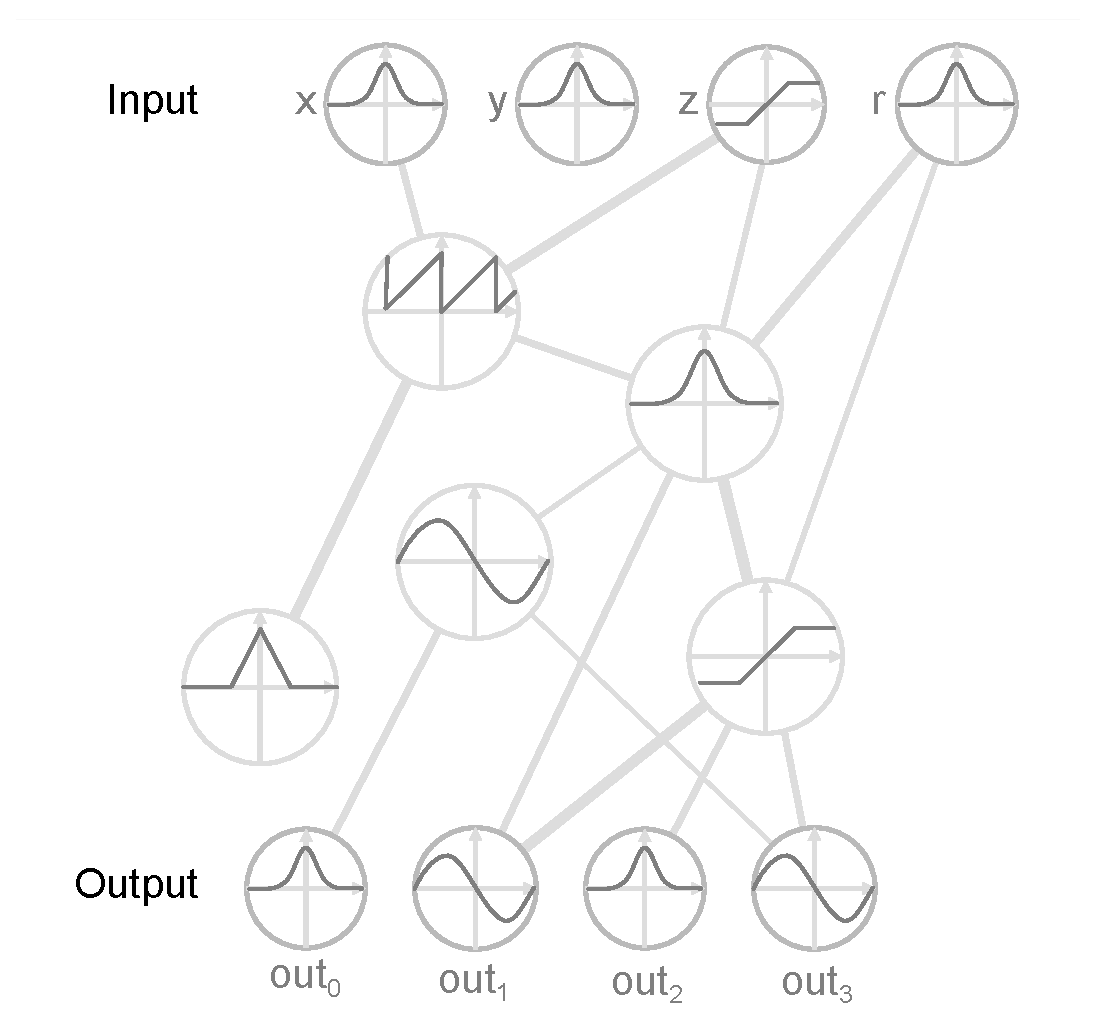
\includegraphics[width=0.6\textwidth]{figure/CPPN}
  \caption{Example of a compositional pattern-producing network. Input is z, y, and z coordinates and r, the radial distance to origo. Each link has a certain weight \(w\) and each node has a certain activation function \(f\). Values are propagated through the network by calculating the next value \(v_{i,t+1}\) of each node as its activation function of the sum of the previous values times weights for all its connected nodes; that is \(v_{i,t+1}=\sum_{j\in n}f(v_{j,t}*w_{ij})\), where \(n\) is the set of nodes connected to node i. A number of outputs is generated for any given location, resulting in a pattern.} \label{fig:cppn} 
\end{figure}

\subsection{Neuroevolution of Augmenting
Topologies} \label{subsec:NEAT}
Neuroevolution, mutating a network topology, is not trivial [ref].  NeuroEvolution of Augmenting Topologies (NEAT) is a method presented by \cite{stanley2002evolving} where a network

In this model, we use the mutations suggested by \cite{stanley2002evolving} and \cite{stanley2007compositional} but disregard crossover since the organisms only reproduce asexually. While crossover could possibly improve the evolution of the organisms, its implementation was left outside the scope of this project.

\tempText{
Explain NEAT mutations: add node, mutate weights, remove connection, add connection. More text to be added here
}

\section{Definition of an organism}
An organism is modelled to consist of three parts:
\begin{enumerate}
    \item The genome, a genotype-to-phenotype mapping structured as a CPPN (see subsection \ref{subsec:CPPN})
    \item The nervous system, an artificial neural network to allow the organism to interact with it's surrounding
    \item A list of the particles that constitutes its cells.
\end{enumerate}
Each cell has a link to its von Neuman neighbours, so that each pair of neighbour particles can exert a spring force holding the organism together.

\subsection{Genome}
The genome consists of a CPPN, as described in \ref{subsec:CPPN}, as well as a discrete vector of organism diameters \(\mathbf{D_{org}}=\left(\begin{array}{ccc} d_x & d_y & d_z \\\end{array}\right)\). An organism consists of at least one cell, placed at the origin and \(\mathbf{D_{org}}\) determines the number of cells outside of it in each direction. Thus, the size of the resulting rectangular cuboid of cells is
\(\mathbf{S_{org}}=\left(\begin{array}{ccc} 2 d_x + 1 & 2 d_y + 1 & 2 d_z + 1 \\\end{array}\right)\).

Given the cell index as input to the CPPN, the resulting output determines the cell type (as well as optional cell properties, for example radius or density), thus defining the organism phenotype.

When an organism reproduces, its genome (and nervous system) will mutate as it is copied to the offspring. The CPPN will mutate according to the NEAT method described in \ref{subsec:NEAT}, while \(\mathbf{D_{org}}\) might increase or decrease in either of its vector components.

\subsection{Nervous system} \label{subsec:nervousSystem}
The nervous system is an ANN (artificial neural network) very similar in structure to the CPPN in the genome and also evolved using the NEAT method (described in \ref{subsec:NEAT}). The input to the nervous system consists of signals from the sensor cells as well as from a bias node sending out a constant value of 1. The output consists of a movement vector for the organism, but could also be expanded to handle other actions such as egg hatching.

\section{Organism coordinate system}
To generate movement from the nervous system output the most simple way would be to generate a force vector \(f=\left(\begin{array}{ccc} f_x & f_y & f_z \\\end{array}\right)\) in the global coordinate system, where the three components of \(f\) are the three output values from the network and \(f\) is added to the current total force of the organism.

However, this approach creates an inherent knowledge of world direction, easily causing the organisms to move, for example: directly up, north or west. As such, the organism in this model instead moves according to their local coordinate system, an approach which will be explained in this section.

\begin{figure}
  \centering
  \includegraphics[width=0.6\textwidth]{figure/neighbours}
  \caption{Identifiers for the six three-dimensional von Neumann neighbours to a cell. Subscripts denote distance in x, y, and z directions between the cell and each neighbour at birth.}
  \label{fig:neighbours} 
\end{figure}

The organisms does not have any stored orientation, since they still consists of relatively independent cells. However, cells have links to their 3-dimensional von Neumann neighbours; front, back, left, right, up and down. These are denoted \(n_{x,y,z}\) as in Figure \ref{fig:neighbours}, where x, y and z are initial distances between the neighbouring cells.

For each neighbour \(n_{x,y,z}\), we then calculate a vector \(v_{x,y,z}\) pointing in their direction as follows:
\[
v_{x,y,z} = 
\begin{cases}
pos(self) - pos(n_{x,y,z}), & \text{if }n_{x,y,z} \text{exists}\\
(0,0,0), & \text{otherwise}
\end{cases}
\]
The function \(pos(n)\) gives the current position of the neighbour \(n\).
Cells at the edges of an organism does not have any neighbours in their "outward" directions, so a zero vector is returned from \(v_{x,y,z}\) if the neighbour does not exist. 

A property of the neighbourhood structure is that the top and bottom neighbour vectors, for example, should point in almost opposite directions. Thus, the six vectors \(v_{0,0,1}, v_{0,0,-1}, ..., v_{-1,0,0}\) can be reduced to three by taking the sum of the linearly dependent pairs:
\begin{align*}
v_x = v_{1,0,0} - v_{-1,0,0}\\
v_y = v_{0,1,0} - v_{0,-1,0}\\
v_z = v_{0,0,1} - v_{0,0,-1}
\end{align*}

These three vectors would work as base vectors defining the local coordinate system of the cell. However, to further account for missing neighbours, each is also combined with the cross product of the other two. Normalized and written as the columns of the transformation matrix \(\mathbb{M}\) we get:

\[
\mathbb{M}=
\left(
\begin{matrix}
 norm(v_x + (v_y \times v_z)), &&
 norm(v_y + (v_z \times v_x)), &&
 norm(v_z + (v_x \times v_y))
\end{matrix}
\right)
\]

Where \(norm(v) = \frac{v}{|v|}\).

Thus from the movement force \(f_{local}\) given by the nervous system in the local coordinate system, we get the force to be applied onto the cell in global coordinates as \(f_{global} = 
c_{move}(\mathbb{M} \cdot f_{local} ) \), where \(c_{move}\) is a movement parameter.

\section{The energy cycle}
The final part of the model to be explained here is the energy cycle; how the energy is transferred through the system. The initial source of energy is the energy particles. Number of energy particles in existence is constant and the number of energy particles entering the simulation volume at any given time step is also close to constant.

This is achieved by, for a simulation volume of height \(h\), initialising the energy particles randomly and, for each energy particle that either gets consumed or reaches the bottom, increase its altitude (y-coordinate) by \(h\) (and setting x- and z-coordinates to a random point within the simulation area).

Energy from the energy particles are then absorbed by photosynthetic cells and spread to their cell neighbours. Different cell types disperse energy in different amounts. For example, egg cells only absorb energy without ever giving anything back, while the energy-harvesting cells part with most of their energy. See Table \ref{tab:cellEnergies} for an example of how the energy dispersion can be configured.

\begin{table}[H]
 \begin{tabular}{| c || c | c | c|} 
    \hline
     Cell type & Energy in & Energy out & Maximum energy \\ [0.5ex] 
     \hline\hline
     Photosynthetic & 0.01 & 0.5 & 10 \\ \hline
     Digestive & 0.01 & 0.5 & 10 \\ \hline
     Sting & 0.01 & 0.5 & 10 \\ \hline
     Vascular & 1 & 0.2 & 3 \\ \hline
     Fat & 1 & 0.01 & 50 \\ \hline
     Sensor & 1 & 0 & 5 \\ \hline
     Buoyancy & 1 & 0 & 5 \\ \hline
     Egg & 1 & 0 & 1000 \\ \hline
 \end{tabular}
\caption{Example of a cell types energy configuration. \emph{Energy in} is the portion of the energy offered by a neighbour that is absorbed,  \emph{Energy out} is the the portion of the cell's surplus energy that is offered to a neighbour.}
\label{tab:cellEnergies}
\end{table}



